\documentclass{article}

\usepackage{graphicx}
\usepackage{tikz}
\usepackage{tikzsymbols}
\usetikzlibrary{calc,patterns,shapes.geometric}
\pagestyle{empty}
\usepackage[margin=0pt]{geometry}
\geometry{papersize={14in,12in}}

\def\centerarc[#1](#2)(#3:#4:#5){\draw[#1] ($(#2)+({#5*cos(#3)},{#5*sin(#3)})$) arc (#3:#4:#5);}

\begin{document}
	\begin{figure}
		\centering
		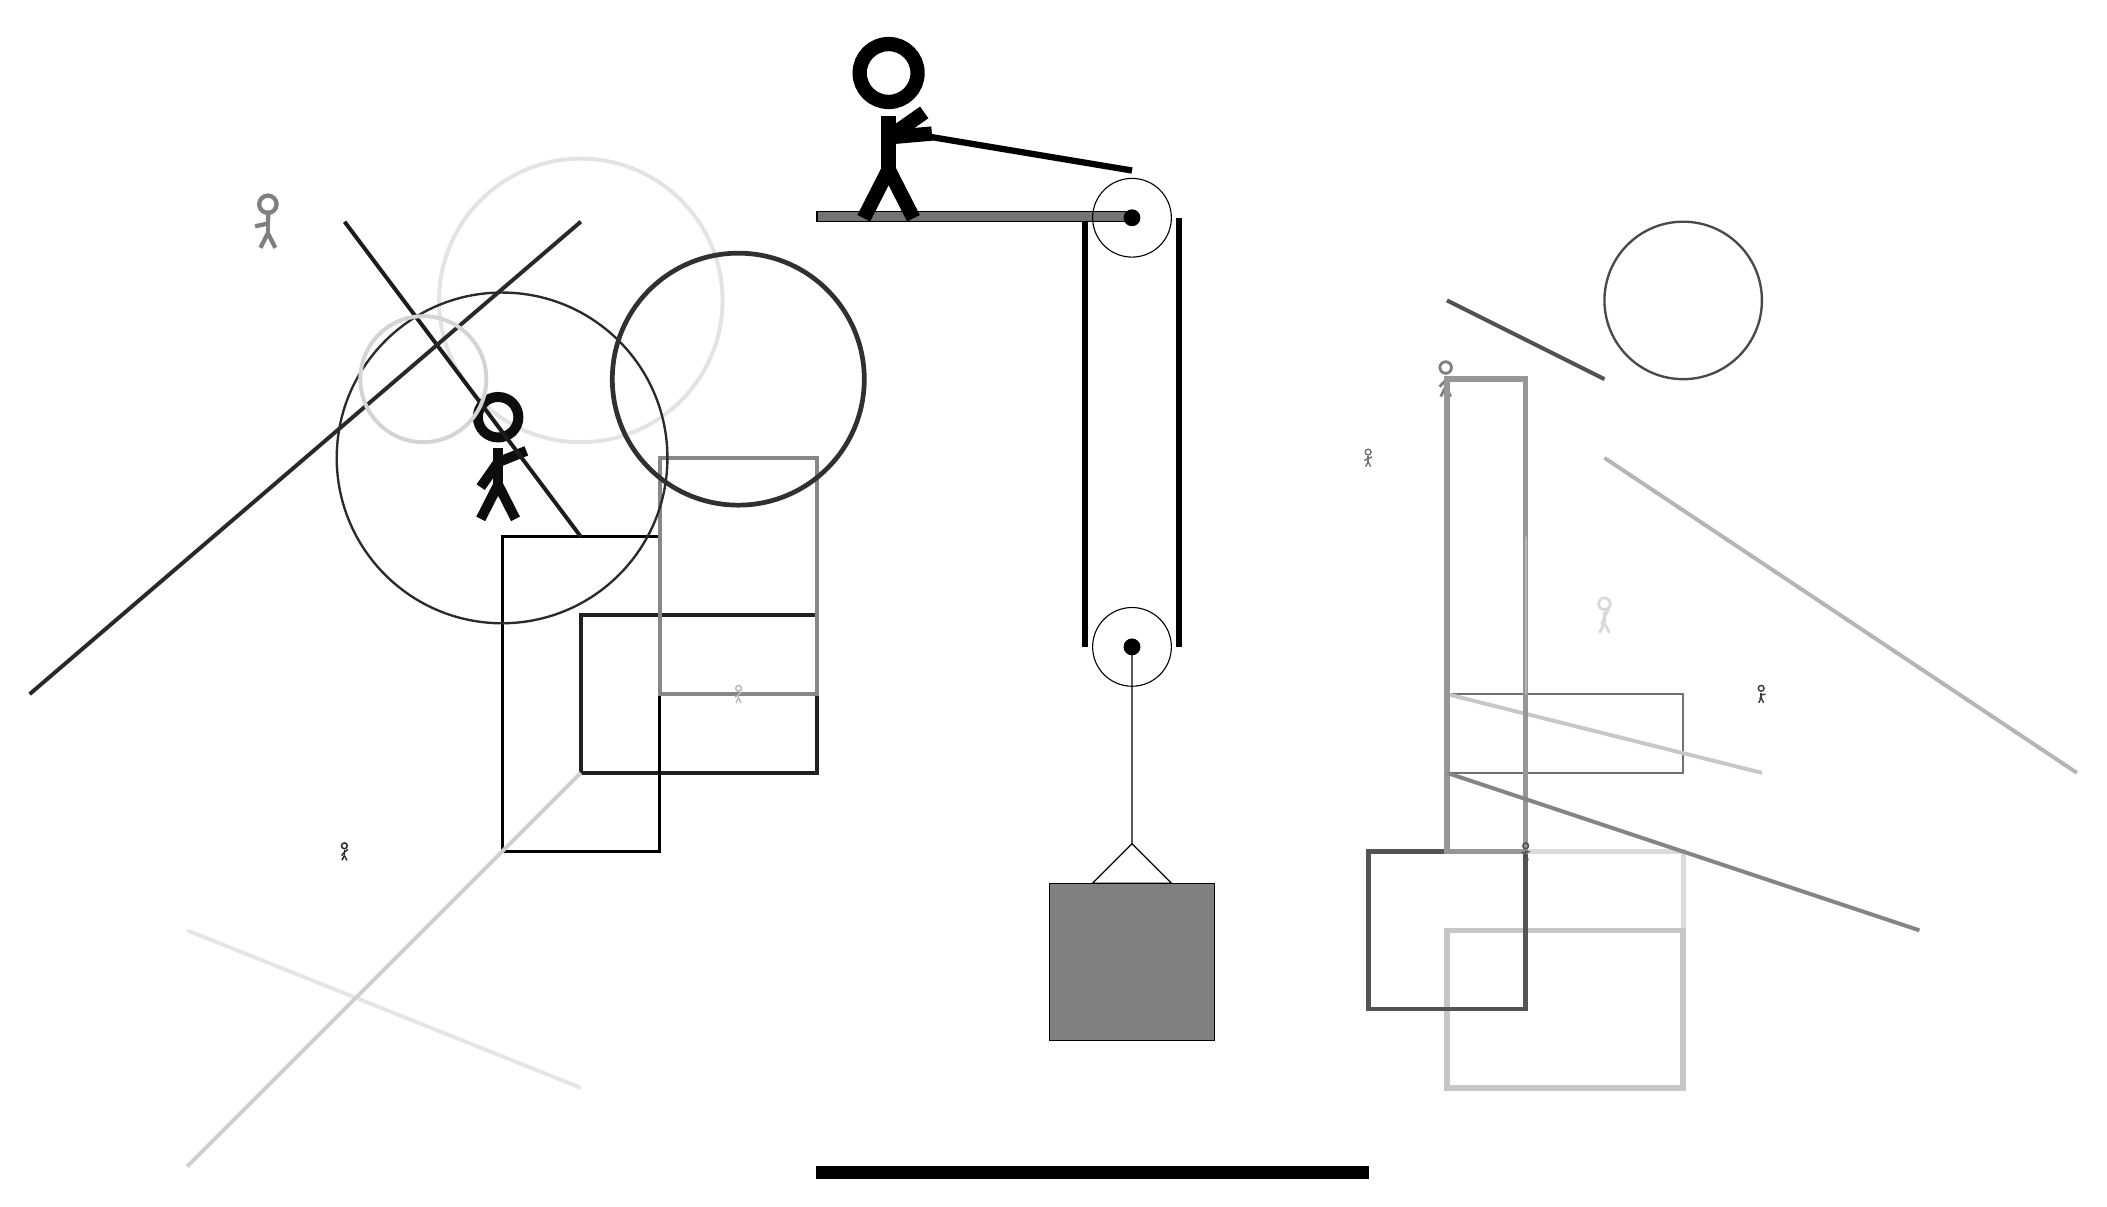
\begin{tikzpicture}
			%%%%% START %%%%%
			
			\draw[fill=black!55] (-2, 9) rectangle (2, 9.125);
			
			\draw (2, 3.6) circle (0.5);
			\draw[fill=black] (2, 3.6) circle (0.1);
			
			\draw (2, 9.05) circle (0.5);
			\draw[fill=black] (2, 9.05) circle (0.1);
			
			\draw (2, 3.6) -- (2, 1.1) -- (1.5, 0.6) -- (2.5, 0.6) -- (2, 1.1);
			\draw[fill=black!50] (0.95, 0.6) rectangle (3.05, -1.4);
			
			\draw[line width=0.8mm] (1.4, 9) -- (1.4, 3.6);
			\centerarc[line width=0.8mm](2, 3.6)(180:360:0.6);
			\draw[line width=0.8mm](2.6, 3.6) -- (2.6, 9.05);
			\centerarc[line width=0.8mm](2, 9.05)(0:90:0.6);
			\draw[line width=0.8mm](2, 9.65) -- (-1, 10.15);
			
			\node[line width=0.7mm, color=black!76] at (10, 3) {\Strichmaxerl[1][74][6]};
			
			\node[line width=0.4mm, color=black!50] at (-9, 9) {\Strichmaxerl[3][12][87]};
			\draw[line width=0.5mm, color=black!87] (-2, 4) rectangle (-5, 2);
			\node[line width=0.6mm, color=black!55] at (5, 6) {\Strichmaxerl[1][26][22]};
			
			\draw [line width=0.5mm, color=black!11](-5, 8) circle (1.8);
			
			\draw[line width=0.4mm, color=black!100] (-4, 5) rectangle (-6, 1);
			\node[line width=0.7mm, color=black!95] at (-6, 6) {\Strichmaxerl[7][55][22]};
			\draw[line width=0.5mm, color=black!68](6, 8) -- (8, 7);
			\draw [line width=0.3mm, color=black!71](9, 8) circle (1.0);
			\draw[line width=0.6mm, color=black!84] (-2, 3) rectangle (-3, 3);
			\draw[line width=0.6mm, color=black!14] (7, 1) rectangle (9, 0);
			\draw[line width=0.5mm, color=black!10](-5, -2) -- (-10, 0);
			\draw[line width=0.5mm, color=black!47] (-4, 3) rectangle (-2, 6);
			
			\draw[line width=0.3mm, color=black!56] (6, 3) rectangle (9, 2);
			\draw[line width=0.5mm, color=black!89](-5, 5) -- (-8, 9);
			\node[line width=0.4mm, color=black!15] at (8, 4) {\Strichmaxerl[2][71][59]};
			
			\draw[line width=0.5mm, color=black!22](10, 2) -- (6, 3);
			
			\node[line width=0.2mm, color=black!29] at (-3, 3) {\Strichmaxerl[1][34][45]};
			\draw[line width=0.7mm, color=black!22] (6, -2) rectangle (9, 0);
			\node[line width=0.4mm, color=black!86] at (-8, 1) {\Strichmaxerl[1][51][40]};
			\draw[line width=0.5mm, color=black!29](8, 6) -- (14, 2);
			\node[line width=0.5mm, color=black!50] at (6, 7) {\Strichmaxerl[2][46][7]};
			\draw[line width=0.6mm, color=black!67] (5, -1) rectangle (7, 1);
			\draw [line width=0.3mm, color=black!83](-6, 6) circle (2.1);
			\draw[line width=0.7mm, color=black!41] (7, 7) rectangle (6, 1);
			
			\draw[line width=0.5mm, color=black!84](-5, 9) -- (-12, 3);
			\draw [line width=0.5mm, color=black!17](-7, 7) circle (0.8);
			\draw [line width=0.6mm, color=black!81](-3, 7) circle (1.6);
			\node[line width=0.4mm, color=black!69] at (7, 1) {\Strichmaxerl[1][10][10]};
			\draw[line width=0.2mm, color=black!28] (7, 5) rectangle (7, 3);
			\draw[line width=0.5mm, color=black!19](-5, 2) -- (-10, -3);
			
			\draw[line width=0.5mm, color=black!48](6, 2) -- (12, 0);
			
			\node at (-1, 10.15) {\Strichmaxerl[10][-175][35]};
			
			\draw[fill=black] (-2, -3) rectangle (5, -3.15);
			
			%%%%% END %%%%%
		\end{tikzpicture}
	\end{figure}	
\end{document}